\documentclass[12pt]{article}

\usepackage[english]{babel}
\usepackage[utf8]{inputenc}
\usepackage{amsmath}
\usepackage{amssymb}
\usepackage{graphicx}
\usepackage{geometry}
\usepackage[colorinlistoftodos]{todonotes}
\usepackage{caption}
    \captionsetup{font=small,labelfont=bf}
\usepackage{enumerate}
\usepackage{lscape}
\usepackage{caption}
\usepackage{verbatim}
\usepackage{csvsimple}

\captionsetup{font={small}}
\geometry{left=2.0cm, right=2.0cm, top=2.5cm, bottom=2.5cm}

\title{Take Home Exam II}

\author{Xingche Guo}

\date{\today}

\linespread{1.3}
\begin{document}
\maketitle

\section{Introduction}
The main purpose of this study is to learn the different parametric methods, (e.g. \textbf{Wald's Theory}, \textbf{Inversion of Likelihood Ratio}, and \textbf{Parametric Bootstrap}), for constructing confident intervals of the parameters in Inverse Gaussian distribution under different conditions (e.g.  differences in sample size $n$ and in dispersion parameter $\lambda$).  On the other hand, this research gives me a chance to practice conducting a Monte Carlo study and to learn how to compare methods by different criteria.\\ 

I'm interested in doing this because this study is very meaningful. The results tells me the pros and cons of these methods under different conditions, which might give me a better idea of selecting methods to conduct confidence intervals. This study also shows how the sample size $n$ and dispersion parameter $\lambda$ affect the confidence interval features. Besides, it sheds light on determining how big the Monte Carlo sample size $M$ and bootstrap sample size $N$ should be, which are all very useful in my later research.













\section{Methods}
\subsection{Method 1}
The density function of an Inverse Gaussian distribution can be written as:
$$f(y|\mu,\lambda)=\sqrt{\frac{\lambda}{2 \pi y^3}} exp(-\frac{\lambda (y-\mu)^2}{2\mu^2 y}); \ \ \ y>0; \ \mu>0; \ \lambda >0$$
Thus, the joint density of iid r.v. $Y_1,\dots, Y_n$ is:
$$f(\pmb{y}|\mu,\lambda)=\prod_{i=1}^{n}f(y_i|\mu,\lambda)$$
The log likelihood function of the joint density is:
\begin{eqnarray*}
l(\mu,\lambda; \pmb{y}) & = & \sum_{i=1}^{n}log\ f(y_i|\mu,\lambda) \\
& = & \sum_{i=1}^{n}(\frac{1}{2}log\frac{\lambda}{2\pi y^3}-\frac{\lambda (y_{i}^2-2y_i \lambda+\mu^2)}{2\mu^2 y_i}) \\
& = & \frac{n}{2}log\lambda -\frac{\lambda}{2\mu^2}\sum_{i=1}^{n}y_i + \frac{n\lambda}{\mu} -\frac{\lambda}{2} \sum_{i=1}^{n} \frac{1}{y_i} - \frac{1}{2} \sum_{i=1}^{n} log\ 2\pi y_{i}^3
\end{eqnarray*}
Compute the MLE by solving:
 \begin{equation*}
\left\{                         
\begin{aligned}
\frac{\partial l}{\partial \mu} &= 0\\
\frac{\partial l}{\partial \lambda} &= 0\\
\end{aligned}
\right.
\end{equation*}

The MLE of $\mu$ and $\lambda$ is:
 \begin{equation*}
\left\{                         
\begin{aligned}
\hat{\mu} &= \frac{\sum_{i=1}^{n}y_i}{n}\\
\hat{\lambda} &=(\frac{\sum_{i=1}^{n} \frac{1}{y_i}}{n}-\frac{n}{\sum_{i=1}^{n}y_i})^{-1}\\
\end{aligned}
\right.
\end{equation*}

The Fisher's Information Matrix is:
 \begin{equation*}
 I(\mu,\lambda)=
\left(                        
\begin{matrix}
\frac{n\lambda}{\mu^3} & 0 \\
0 & \frac{n}{2\lambda^2}
\end{matrix}
\right)
\end{equation*}

By Wald's theory, the $95\%$ Confidence Interval of $\mu$ and $\lambda$ is: 
 \begin{equation*}
\left\{                         
\begin{aligned}
\mu &\in \hat{\mu} \pm 1.96 \times \sqrt{\frac{\hat{\mu}^3}{n\hat{\lambda}}}\\
\lambda &\in \hat{\lambda} \pm 1.96 \times \sqrt{\frac{2\hat{\lambda}^2}{n}}\\
\end{aligned}
\right.
\end{equation*}

\subsection{Method 2}
For $\lambda$, using the profile likelihood thought, define: $l_1(\lambda)=l(\hat{\mu},\lambda)$. By Wilk's theorem, we have:
$$-2(l_1(\lambda_0)-l_1(\hat{\lambda}))\sim \chi_{1}^2, \ when \ n \to \infty .$$
Thus, by the inversion of likelihood ratio statistics, the $95\%$ Confidence Interval of $\lambda$ is: 
$$\{  \lambda \in R^{+}:  -2(l_1(\lambda)-l_1(\hat{\lambda}))  \leq    \chi_{1}^2 (0.95) \}$$

Define: 
$$T_{\lambda} = -2(l_1(\lambda)-l_1(\hat{\lambda}))$$
Then:
\begin{eqnarray*}
T_{\lambda} &=& -2[(  \frac{n}{2}log\lambda + \frac{n\lambda}{2\hat{\mu}} -\frac{\lambda}{2} \sum_{i=1}^{n} \frac{1}{y_i}  )-(  \frac{n}{2}log\hat{\lambda} + \frac{n\hat{\lambda}}{2\hat{\mu}} -\frac{\hat{\lambda}}{2} \sum_{i=1}^{n} \frac{1}{y_i}  )] \\
&=& (\sum_{i=1}^{n}\frac{1}{y_i}-\frac{n}{\hat{\mu}})(\lambda-\hat{\lambda})-n log\ \frac{\lambda}{\hat{\lambda}}
\end{eqnarray*}
\\
\\
\\
For $\mu$, notice that:
$$\frac{\partial l}{\partial \lambda}=0 \ \ \to \lambda = (\frac{\hat{\mu}}{\mu^2}-\frac{2}{\mu}+\frac{\sum_{i=1}^{n}\frac{1}{y_i}}{n})^{-1}$$
So, we define:
$$\tilde{\lambda} \equiv \tilde{\lambda}(\mu)=(\frac{\hat{\mu}}{\mu^2}-\frac{2}{\mu}+\frac{\sum_{i=1}^{n}\frac{1}{y_i}}{n})^{-1}$$
Then define: $l_2(\mu)=l(\mu,\tilde{\lambda})$, similarly,  the $95\%$ Confidence Interval of $\mu$ is: 
$$\{  \mu \in R^{+}:  -2(l_2(\mu)-l_2(\hat{\mu}))  \leq    \chi_{1}^2 (0.95) \}$$
Define:
$$T_{\mu} = -2(l_2(\mu)-l_2(\hat{\mu}))$$
Then:
$$T_{\mu}=-2[( \frac{n}{2}log\tilde{\lambda} -\frac{\tilde{\lambda}}{2\mu^2}\sum_{i=1}^{n}y_i + \frac{n\tilde{\lambda}}{\mu} -\frac{\tilde{\lambda}}{2} \sum_{i=1}^{n} \frac{1}{y_i}  )-( \frac{n}{2}log\hat{\lambda} + \frac{n\hat{\lambda}}{2\hat{\mu}} -\frac{\hat{\lambda}}{2} \sum_{i=1}^{n} \frac{1}{y_i} )]$$


To draw a conclusion, the $95\%$ Confidence Interval of $\mu$ and $\lambda$ is: 
 \begin{equation*}
\left\{                         
\begin{aligned}
\mu &\in \{  \mu \in R^{+}:  T_{\mu}  \leq    \chi_{1}^2 (0.95) \}\\
\lambda &\in \{  \lambda \in R^{+}:  T_{\lambda}  \leq    \chi_{1}^2 (0.95) \}\\
\end{aligned}
\right.
\end{equation*}
where $T_{\mu}$ and $T_{\lambda}$ are defined above. \\

These intervals were computed by evaluating the normed profile likelihood for a sequence of values between $lb$ and $ub$ with spacing of 0.001, where $lb$ and $ub$ are functions with respect to the sample size $n$ and the confidence interval width computed by the first method.\\

For example, for the CI of $\mu$, the CI computed by the first method is: $\hat{\mu} \pm 1.96 \times \sqrt{\frac{\hat{\mu}^3}{n\hat{\lambda}}}$. Then we can let:
$$lb = \hat{\mu} -  1.96 \times \sqrt{\frac{\hat{\mu}^3}{n\hat{\lambda}}} \times C_{\mu}(n)$$
$$ub = \hat{\mu} +  1.96 \times \sqrt{\frac{\hat{\mu}^3}{n\hat{\lambda}}} \times C_{\mu}(n)$$
Where $C_{\mu}(n)$ is a function of $n$. By simulation, I decide to use:
 \begin{equation*}
 C_{\mu}(n)=
\left\{                         
\begin{aligned}
15 , \ & n \leq 20 \\
10 , \ & 20 < n \leq 50\\
5 , \ & 50 < n \leq 100\\
3 , \ & 100 < n \leq 200\\
2 , \ & n>200\\
\end{aligned}
\right. \ \ \ \ ;  \ \ \ 
 C_{\lambda}(n)=
\left\{                         
\begin{aligned}
5 , \ & n \leq 20 \\
3 , \ & 20 < n \leq 50\\
2 , \ & n>50\\
\end{aligned}
\right.
\end{equation*}
\\
Notice that this bound-decide method will get a narrower CI width of $\mu$ compared with the theoretical one when $n=10$. However, since the true coverage rate is very close to 0.95, the narrower CI width will lead to a better performance. On the other hand, our bound-decide method would be much faster when n become larger than the bound-decide method that is unified for different sample size $n$.\\

\subsection{Method 3}
By Maximum likelihood and parametric bootstrap using the comparison function: $h(\theta,\hat{\theta})=n^{1/2}(\hat{\theta}-\theta)$. We can write down the algorithm as follow:
\begin{itemize}
  \item Step1: Calculate $\hat{\mu}$ and $\hat{\lambda}$ (the MLE of $\mu$ and $\lambda$ using the original data).
  \item Step2: Generate observations $\pmb{y_{m}^{*}}=(y_{1m}^{*},\dots,y_{nm}^{*}), \ m=1,\dots,N$, from the fitted model $Inv.Gauss(\hat{\mu},\hat{\lambda})$. ($N$ will be decided later).
  \item Step3: Calculate $\mu_{m}^{*}$ and $\lambda_{m}^{*}$ (the MLE of $\mu$ and $\lambda$ using the $m$th generated data).
  \item Step4: Calculate $\mu_{[(N+1)(0.025)]}^{*}$, $\mu_{[(N+1)(0.975)]}^{*}$, $\lambda_{[(N+1)(0.025)]}^{*}$, $\lambda_{[(N+1)(0.975)]}^{*}$ (e.g. $\mu_{[(N+1)(0.025)]}^{*}$ is the [(N+1)(0.025)]th order statistics of $\{\mu_{m}^{*}\}_{m=1}^{N}$).
\end{itemize}

Then the $95\%$ Confidence Interval of $\mu$ and $\lambda$ is: 
 \begin{equation*}
\left\{                         
\begin{aligned}
\mu &\in (2\hat{\mu}-\mu_{[(N+1)(0.975)]}^{*},2\hat{\mu}-\mu_{[(N+1)(0.025)]}^{*})\\
\lambda &\in (2\hat{\lambda}-\lambda_{[(N+1)(0.975)]}^{*},2\hat{\lambda}-\lambda_{[(N+1)(0.025)]}^{*}).\\
\end{aligned}
\right.
\end{equation*}


\subsection{Method 4}
By Maximum likelihood and parametric bootstrap using the comparison function: $h(\theta,\hat{\theta})=n^{1/2}(\frac{\theta}{\hat{\theta}}-1)$. The algorithm is the same as in Method 3.

The $95\%$ Confidence Interval of $\mu$ and $\lambda$ is: 
 \begin{equation*}
\left\{                         
\begin{aligned}
\mu &\in (\frac{\hat{\mu}^2}{\mu_{[(N+1)(0.975)]}^{*}},\frac{\hat{\mu}^2}{\mu_{[(N+1)(0.025)]}^{*}})\\
\lambda &\in (\frac{\hat{\lambda}^2}{\lambda_{[(N+1)(0.975)]}^{*}},\frac{\hat{\lambda}^2}{\lambda_{[(N+1)(0.025)]}^{*}}).\\
\end{aligned}
\right.
\end{equation*}



\subsection{Method 5}
By Maximum likelihood and parametric bootstrap using the comparison function: $h(\theta,\hat{\theta})=\frac{\hat{\theta}-\theta}{V(\hat{\theta})^{1/2}}$. Only step 4 of the algorithm will change. We now need to calculate $(\frac{\theta^{*}-\hat{\theta}}{V(\theta^{*})^{1/2}})_{[(N+1)(0.025)]}$ and $(\frac{\theta^{*}-\hat{\theta}}{V(\theta^{*})^{1/2}})_{[(N+1)(0.975)]}$ instead of $\theta^{*}_{[(N+1)(0.025)]}$ and $\theta^{*}_{[(N+1)(0.975)]}$, where $\theta$ denote $\mu$ or $\lambda$.

Thus, the $95\%$ Confidence Interval of $\mu$ and $\lambda$ is: 
 \begin{equation*}
\left\{                         
\begin{aligned}
\mu &\in (\hat{\mu}-[V(\hat{\mu})]^{1/2}(\frac{\mu^{*}-\hat{\mu}}{V(\mu^{*})^{1/2}})_{[(N+1)(0.975)]},\hat{\mu}-[V(\hat{\mu})]^{1/2}(\frac{\mu^{*}-\hat{\mu}}{V(\mu^{*})^{1/2}})_{[(N+1)(0.025)]})\\
\lambda &\in (\hat{\lambda}-[V(\hat{\lambda})]^{1/2}(\frac{\lambda^{*}-\hat{\lambda}}{V(\lambda^{*})^{1/2}})_{[(N+1)(0.975)]},\hat{\lambda}-[V(\hat{\lambda})]^{1/2}(\frac{\lambda^{*}-\hat{\lambda}}{V(\lambda^{*})^{1/2}})_{[(N+1)(0.025)]}).\\
\end{aligned}
\right.
\end{equation*}

Where:
$$V(\tilde{\mu})=\frac{\tilde{\mu}^3}{n \tilde{\lambda}} \ ; \ \ \ \ V(\tilde{\lambda})=\frac{2\tilde{\lambda}^2}{n}.$$

($\tilde{\mu}$ denotes $\hat{\mu}$ or $\mu^{*}$,  $\tilde{\lambda}$ denotes $\hat{\lambda}$ or $\lambda^{*}$).
\\
Note that: 
\begin{eqnarray*}
&&\hat{\lambda}-[V(\hat{\lambda})]^{1/2}(\frac{\lambda^{*}-\hat{\lambda}}{V(\lambda^{*})^{1/2}})_{[(N+1)(0.975)]}\\
&=&\hat{\lambda}-\sqrt{\frac{2}{n}}\hat{\lambda}(\frac{\lambda^{*}-\hat{\lambda}}{\sqrt{\frac{2}{n}}\lambda^*})_{[(N+1)(0.975)]}\\
&=&\hat{\lambda}-\hat{\lambda}(1-\frac{\hat{\lambda}}{\lambda^*})_{[(N+1)(0.975)]}\\
&=&\hat{\lambda}-\hat{\lambda}(1-\frac{\hat{\lambda}}{\lambda^{*}_{[(N+1)(0.975)]}})\\
&=&\frac{\hat{\lambda}^2}{\lambda_{[(N+1)(0.975)]}^{*}}.\\
\end{eqnarray*}

Similarly:
\begin{eqnarray*}
&&\hat{\lambda}-[V(\hat{\lambda})]^{1/2}(\frac{\lambda^{*}-\hat{\lambda}}{V(\lambda^{*})^{1/2}})_{[(N+1)(0.025)]}\\
&=&\frac{\hat{\lambda}^2}{\lambda_{[(N+1)(0.025)]}^{*}}.\\
\end{eqnarray*}

Hence, method 4 and method 5 will have the same Confidence Interval for $\lambda$ given the same seed of randomness. 

\subsection{Method 6}
By Method of Moment estimation and parametric bootstrap using the comparison function: $h(\theta,\hat{\theta})=n^{1/2}(\hat{\theta}-\theta)$. The algorithm will be similar, the only difference is to replace all the $\hat{\mu}$ and $\hat{\lambda}$ by $\mu_{MME}$ and $\lambda_{MME}$.

 \begin{equation*}
\left\{                         
\begin{aligned}
\mu_{MME} &=\frac{1}{n} \sum_{i=1}^{n}Y_i \\
\lambda_{MME} &= \frac{\mu_{MME}^3}{\frac{1}{n} \sum_{i=1}^{n}Y_{i}^2 -  \mu_{MME}^2}. \\
\end{aligned}
\right.
\end{equation*}

Thus, the $95\%$ Confidence Interval of $\mu$ and $\lambda$ is: 
 \begin{equation*}
\left\{                         
\begin{aligned}
\mu &\in (2\mu_{MME}-\mu_{MME,[(N+1)(0.975)]}^{*},2\mu_{MME}-\mu_{MME,[(N+1)(0.025)]}^{*})\\
\lambda &\in (2\lambda_{MME}-\lambda_{MME,[(N+1)(0.975)]}^{*},2\lambda_{MME}-\lambda_{MME,[(N+1)(0.025)]}^{*}).\\
\end{aligned}
\right.
\end{equation*}



\subsection{R Functions and Packages Used}


\begin{itemize}
  \item Generate Inverse Gaussian distribution: \textbf{statmod::rinvgauss(x, mean, shape)}.
    \item All the other R functions are written by me (In Appendix).
\end{itemize}



\subsection{Choose Bootstrap --- N}
There are too many combinations of experiments: $\lambda \in \{2,4,8,12\}$, $n \in \{10,25,50,100,500\}$, $method \in \{3,4,5,6\}$. It's not efficient to find the best N for all these combinations. So, I use the thought of "Latin Square Design" to compute the confidence interval width of the following combinations when $N \in \{50,100,200,300,\dots,10000\}$. The results are in figure[1] and figure[2] in the Appendix.\\

\begin{tabular}{|c|cccc|}
\hline
  & method3 & method4 & method5 & method6\\
 \hline
$\lambda=2$ & n=10 & n=50 & n=100 & n=500 \\
$\lambda=4$ & n=50 & n=100 & n=500 & n=10 \\
$\lambda=8$ & n=100 & n=500 & n=10 & n=50 \\
$\lambda=12$ & n=500 & n=10 & n=50 & n=100\\
\hline
\end{tabular}
\\



The figure[1] and figure[2] show that the CI widths converge for most of the combinations when N=2000. Thus, we pick the bootstrap N to be 2000.\\




\subsection{Choose Monte Carlo --- M}
In order to make the comparison between different combinations of experiments, we need to find one unified M. In this case, I compute:
\begin{itemize}
 \item the coverage rate of $\mu$:  given $n=100$ and $method=1$ for the four different $\lambda$ (figure[3]);
 \item the coverage rate of $\mu$:  given $\lambda=4$ and $method=1$ for the five different $n$ (figure[4]);
 \item the coverage rate of $\mu$:  given $\lambda=4$ and $n=10$  for the six different methods (figure[5]);
 \end{itemize}

I also compute the coverage rate of $\lambda$ in the same conditions, the results are similar. By checking the figures, I find the coverage rates become stable when $\sqrt{M}=100$, which means $M=10000$. So, I choose M to be 10000 for all the cases.\\


\subsection{Monte Carlo Study Algorithm }
\textbf{------------to Calculate the 3 Criteria of Confidence Intervals Computed by each Methods.} (when $\mu_0 =5$, $n_0 \in \{10,25,50,100,500\}$, $\lambda_0 \in \{2,4,8,12\}$),$method \in \{1,2,3,4,5,6\}$).\\
 \\
 \\
 \textbf{for} ($i \ \in \ 1:10000$)\{\\
  $\blacklozenge$ Generate $n_0$ Inverse Gaussian r.v. of $\mu=\mu_0$ and $\lambda=\lambda_0$ \\
  by R function \textbf{statmod::rinvgauss($n$,\ $\mu$,\ $\lambda$)}.\\
$\blacklozenge$ Compute $95\%$ CI: $I_{\mu}^{(i)}$, $I_{\lambda}^{(i)}$  using the algorithm in Section 2.1---2.6\\
 and the R function in Appendix 5.1. (N = 2000 when using method 3---6)\\
\}\\
\\
$\blacklozenge$ Compute the actual coverage rate by:
 $$cv_{\mu}=\frac{1}{10000}\sum_{i=1}^{10000}I(\mu_0 \in I_{\mu}^{(i)}); \ \ cv_{\lambda}=\frac{1}{10000}\sum_{i=1}^{10000}I(\lambda_0 \in I_{\lambda}^{(i)}).$$
$\blacklozenge$ Compute the median width simply by the R median function.\\
$\blacklozenge$ Compute the out of bound probability by:
 $$P_{\mu}=\frac{1}{10000}\sum_{i=1}^{10000}I(lower\ bound\ of\ I_{\mu}^{(i)} \leq 0); \ \ P_{\lambda}=\frac{1}{10000}\sum_{i=1}^{10000}I(lower\ bound\ of\ I_{\lambda}^{(i)} \leq 0).$$
\\
\\
\\
The code can be found in Appendix 5.2.\\


\section{Results}

The \textbf{coverage rate}, \textbf{median CI width} and the \textbf{out of bound probability} of all the combinations of experiments ($\lambda \in \{2,4,8,12\}$, $n \in \{10,25,50,100,500\}$, and $method \in \{1,2,3,4,5,6\}$) are shown in table[1] --table[6] in the Appendix. There are also four figures about the coverage rate and median CI width for $\mu$ and $\lambda$ (figure[6] --- figure[9]).







\section{Discussion and Conclusions}
\subsection{Performance of Methods When $n$ Different}
\textbf{For confidence intervals of $\mu$}:\\
 When the sample size $n$ small, the actual coverage rate of method 1, 3, and 6 are small, (i.e. when $n=10$, $\lambda=2$: $cv1=0.7941$, $cv3=0.7339$, $cv6=0.7042$) while the coverage rate of method 2 are very close to 0.95 (i.e. when $n=10$, $\lambda=2$: $cv2=0.9324$). However, the median width of method 2 is too large compared to the other methods (i.e. when $n=10$, $\lambda=2$: $med.wid2=45.7270$, $med.wid1=7.4000$).  I guess the coverage rate of method 2 is close to 0.95 because the CI computed by method 2 is too wide so that the true $\mu$ falls into most of the CI, while the coverage rate of method 1, 3, and 6 is small means the CI computed by these methods are not wide enough to capture enough information.  So, by the coverage rate and median width trade-off, I prefer to pick method 4 and method 5 (i.e. when $n=10$, $\lambda=2$:  $cv4=0.8583$, $cv5=0.8860$, $med.wid4=8.4691$, $med.wid5=13.4934$). Besides, the out of bound probability of method 4 and method 5 is always $0$, which also means method 4 and method 5 are better.\\

When the sample size $n$ large, the differences between the different methods become less. when $n=500$, the differences of the first five methods are nearly negligible (The coverage rate of method 6 when $n=500$ is a little small than the first five methods) and all of the coverage rate of the six methods are approaching to 0.95. So, the first five methods (even method 6) are applicable. In this case, I prefer method 1 because it's the fastest method. \\

\textbf{For confidence intervals of $\lambda$}:\\
Firstly, we should notice a fact that the confidence interval computed by method 4 and method 5 are the same give the same seed. (It has been discussed in section 2.5.)  Also, the results of method 1 and method 2 perform very similar (nearly the same) by checking table [2], [4], and [6].\\

When the sample size $n$ small,  method 1, 2, 4, and 5 have the similar median CI width, method 3 and method 6 have a much larger median CI width than the front four methods. (i.e. when $n=10$, $\lambda=2$:  $med.wid1=4.1874$, $med.wid2=4.276$, $med.wid4\&5=3.9031$, $med.wid3=7.5531$, $med.wid6=17.6629$). On the other hand, the out of bound probability of method 3 and method 6 are very large while the other four methods always have 0 probability (i.e. when $n=10$, $\lambda=2$:  $P(out \ of \ bound\ of \ method \ 3)=1$, $P(out \ of \ bound\ of \ method \ 6)=1$).  In the table [2], I notice that the coverage rate of method 4 and 5 are closer to 0.95 than method 1 and 2, while the confidence intervals are narrower. In this case, I recommend to choose method 4 or method 5. (Method 4 is a little faster).\\

When the sample size $n$ large, the first five methods outperform the method 6 (i.e. when $n=500$, $\lambda=2$: the median width of the first fives methods are about 0.497, while $med.wid6 = 1.3649$). Besides, the out of bound probability of method 6 when $n=100$, $\lambda=2$ is still big (i.e. P=0.1697). As a result, first five methods are applicable. In this case, I prefer method 1 because it's the fastest.\\

\subsection{Performance of Methods When $\lambda$ Different}
The change of $\lambda$ will not affect the performance of the confidence interval for $\lambda$, however, it does have influence on the confidence interval for $\mu$. It can be found in table [1], [3] and [5] that the performance of the confidence interval for $\mu$ becomes better when $\lambda$ increase (i.e. the coverage rate is closer to 0.95, the out of bound probability is smaller).  \\

By checking table [1], I found the coverage rate of method 2 and method 5 for $\mu$ is closer to 0.95 than the other four methods when $\lambda$ is large and $n$ is small (e.g. when $n=10$, $\lambda=12$: $cv2=0.9282$, $cv5=0.9376$, the other methods are all less than 0.9). At the same time, the median CI width of these two methods are not too large compared to the other four methods, the out of bound probability is 0 for these two methods. So, I would like to pick method 2 or method 5 for conducting CI of $\mu$ when $\lambda$ large and $n$ small. \\

The method 4 is also applicable since the out of bound probability is 0 and the coverage rate is higher than method 1, 3 and 6, though it's not as good as method 2 and method 5.\\


\subsection{Checking the figure [6]---[9]}
The discussion above is based on the table [1]---[6], we can get the same conclusion by check the figure [6]---[9], which are more clear than the tables.\\

For the CI for $\mu$, note that the coverage rate given by the method 2, 4, and 5 converge faster than method 1, 3 and 6. However, the median width computed by method 2 is much larger than the other ones when $\lambda$ is small. Thus, the method 4 and 5 is preferable. Method 2 is applicable when $\lambda$ is large. When $n$ is large, the coverage rate and median width for all of the methods become very close. \\

For the CI for $\lambda$, note that the median width for method 1, 2, 4, and 5 are very close and they are smaller than the median width for method 3 and 6. On the other hand, the coverage rate computed by method 4 and 5 are closest to 0.95 among all methods. Thus, method 4 and 5 are better. When n is large, the coverage rate and median width for the first 5 methods become very close. \\




\subsection{Conclusions}

For the confidence interval of $\mu$, the following methods have good performance (* The method in bracket means: applicable but not as good as the other ones.):\\

\begin{tabular}{|c|c|c|}
\hline
  & $n$ small & $n$ large\\
 \hline
$\lambda$ small & method 4  5 &  method 1 2 3 4 5 (6)\\
$\lambda$ large & method 2 (4) 5 & method 1 2 3 4 5 (6)\\
\hline
\end{tabular}
\\
\\

For the confidence interval of $\lambda$, the following methods have good performance:\\

\begin{tabular}{|c|c|}
\hline
  $n$ small & $n$ large\\
 \hline
method 4 5  &  method 1 2 3 4 5\\
\hline
\end{tabular}
\\
\\

Over all, my favorite method is method 5 since it has a good performance in any condition.  Method 4 is also a reasonable choice. However, I recommend to use method 1 when the sample size is large since it's much faster than the other ones. \\

\newpage

\section{Apprendix}
\subsection{R Functions of Method 1-6}

\noindent\makebox[\linewidth]{\rule{\textwidth}{1pt}}
\verbatiminput{method1_6.R}
\noindent\makebox[\linewidth]{\rule{\textwidth}{1pt}}

\subsection{R Functions of 3 criteria}
\noindent\makebox[\linewidth]{\rule{\textwidth}{1pt}}
\begin{verbatim}
  criteria <- function(M,n = 10, mu = 5,lambda = 2,
   para = c("mu","lambda"), method = c(1,2,3,4,5,6)){
    if (method == 1){
    ci_mu <- function(x) ci_mu_1(x)
    ci_la <- function(x) ci_la_1(x)
  }
  if (method == 2){
    ci_mu <- function(x) ci_mu_2(x)
    ci_la <- function(x) ci_la_2(x)
  }
  if (method == 3){
    ci_mu <- function(x) ci_boot_mu_1(x,2000)
    ci_la <- function(x) ci_boot_la_1(x,2000)
  }
  if (method == 4){
    ci_mu <- function(x) ci_boot_mu_2(x,2000)
    ci_la <- function(x) ci_boot_la_2(x,2000)
  }
  if (method == 5){
    ci_mu <- function(x) ci_boot_mu_3(x,2000)
    ci_la <- function(x) ci_boot_la_3(x,2000)
  }
  if (method == 6){
    ci_mu <- function(x) ci_boot_mu_4(x,2000)
    ci_la <- function(x) ci_boot_la_4(x,2000)
  }
    set.seed(520520)
    library(statmod)
    if (para == "mu"){
      IG <- matrix(rinvgauss(M*n,mu,lambda), ncol=M)
      CImu <- apply(IG,2,ci_mu)
      ID <- (CImu[1,]<mu)&(CImu[2,]>mu)
      CI <- t(CImu)
    }
    
    if (para == "lambda"){
      IG <- matrix(rinvgauss(M*n,mu,lambda), ncol=M)
      CIla <- apply(IG,2,ci_la)
      ID <- (CIla[1,]<lambda)&(CIla[2,]>lambda)
      CI <- t(CIla)
    }
    
    rate <- mean(ID)
    width <- CI[,2]-CI[,1]
    med_width <- median(width)
    prob <- mean(CI[,1]<0)
    result <- list(rate = rate,medianWidth = med_width, Prob = prob)
    return(result)
  }
\end{verbatim}
\noindent\makebox[\linewidth]{\rule{\textwidth}{1pt}}

\subsection{Some Tables and Figures}

\begin{figure}[h] 
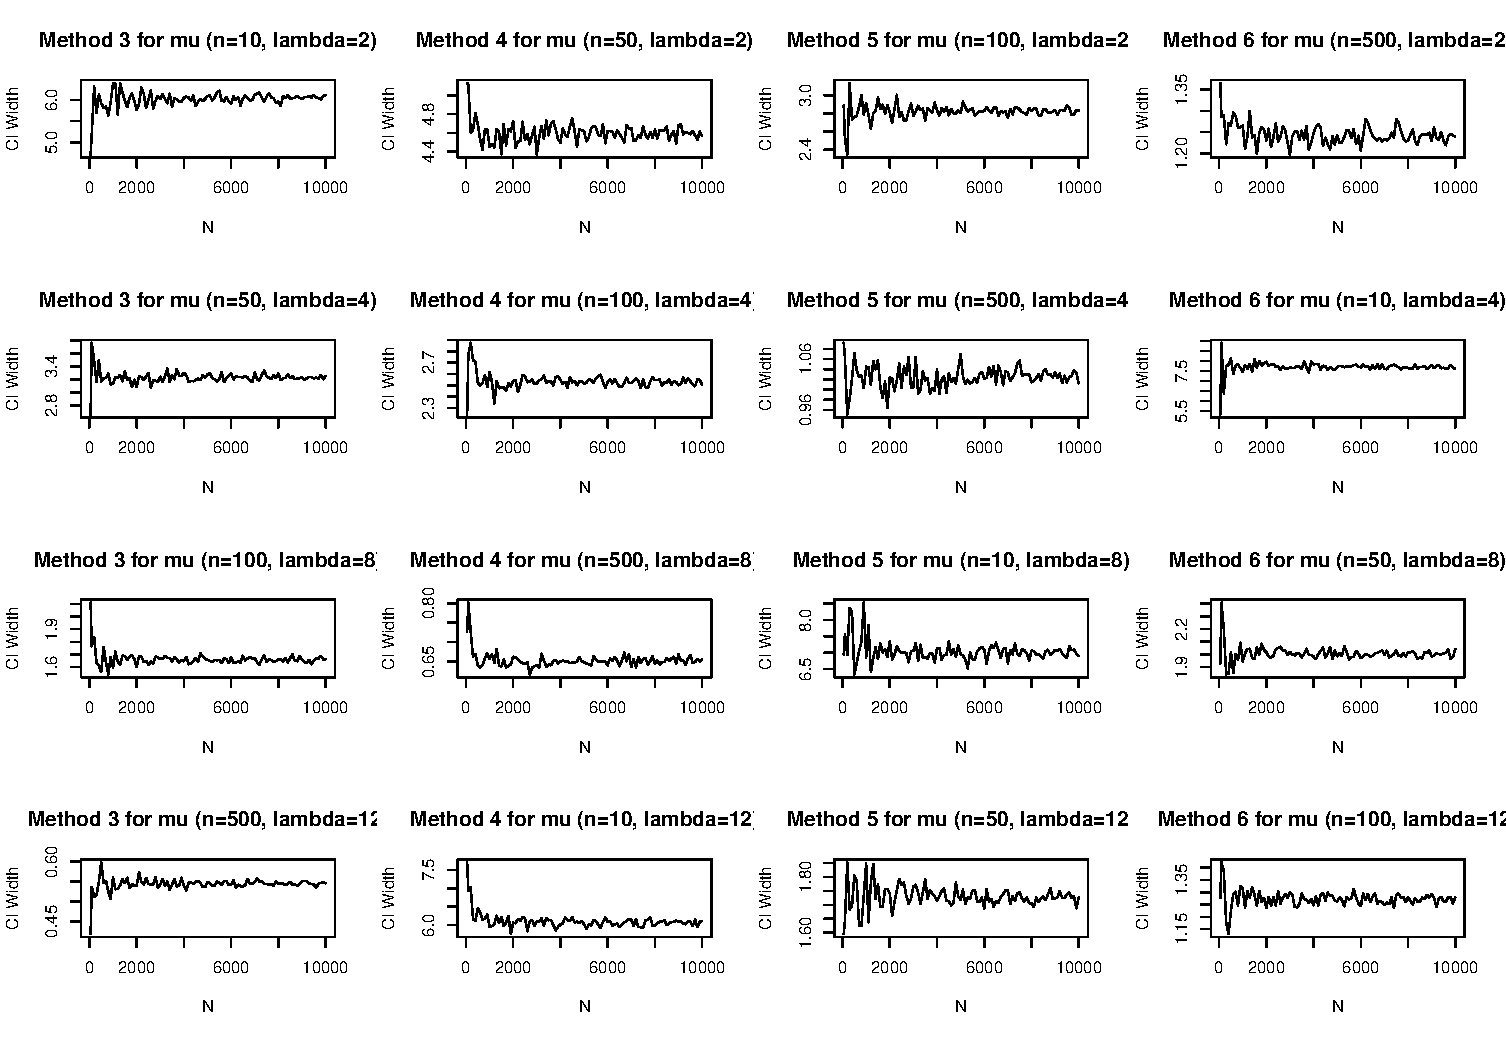
\includegraphics[width=1.0\textwidth]{findN_mu.pdf}
\caption{Choose bootstrap N using the CI width of $\mu$}
\end{figure}



\begin{figure}[h] 
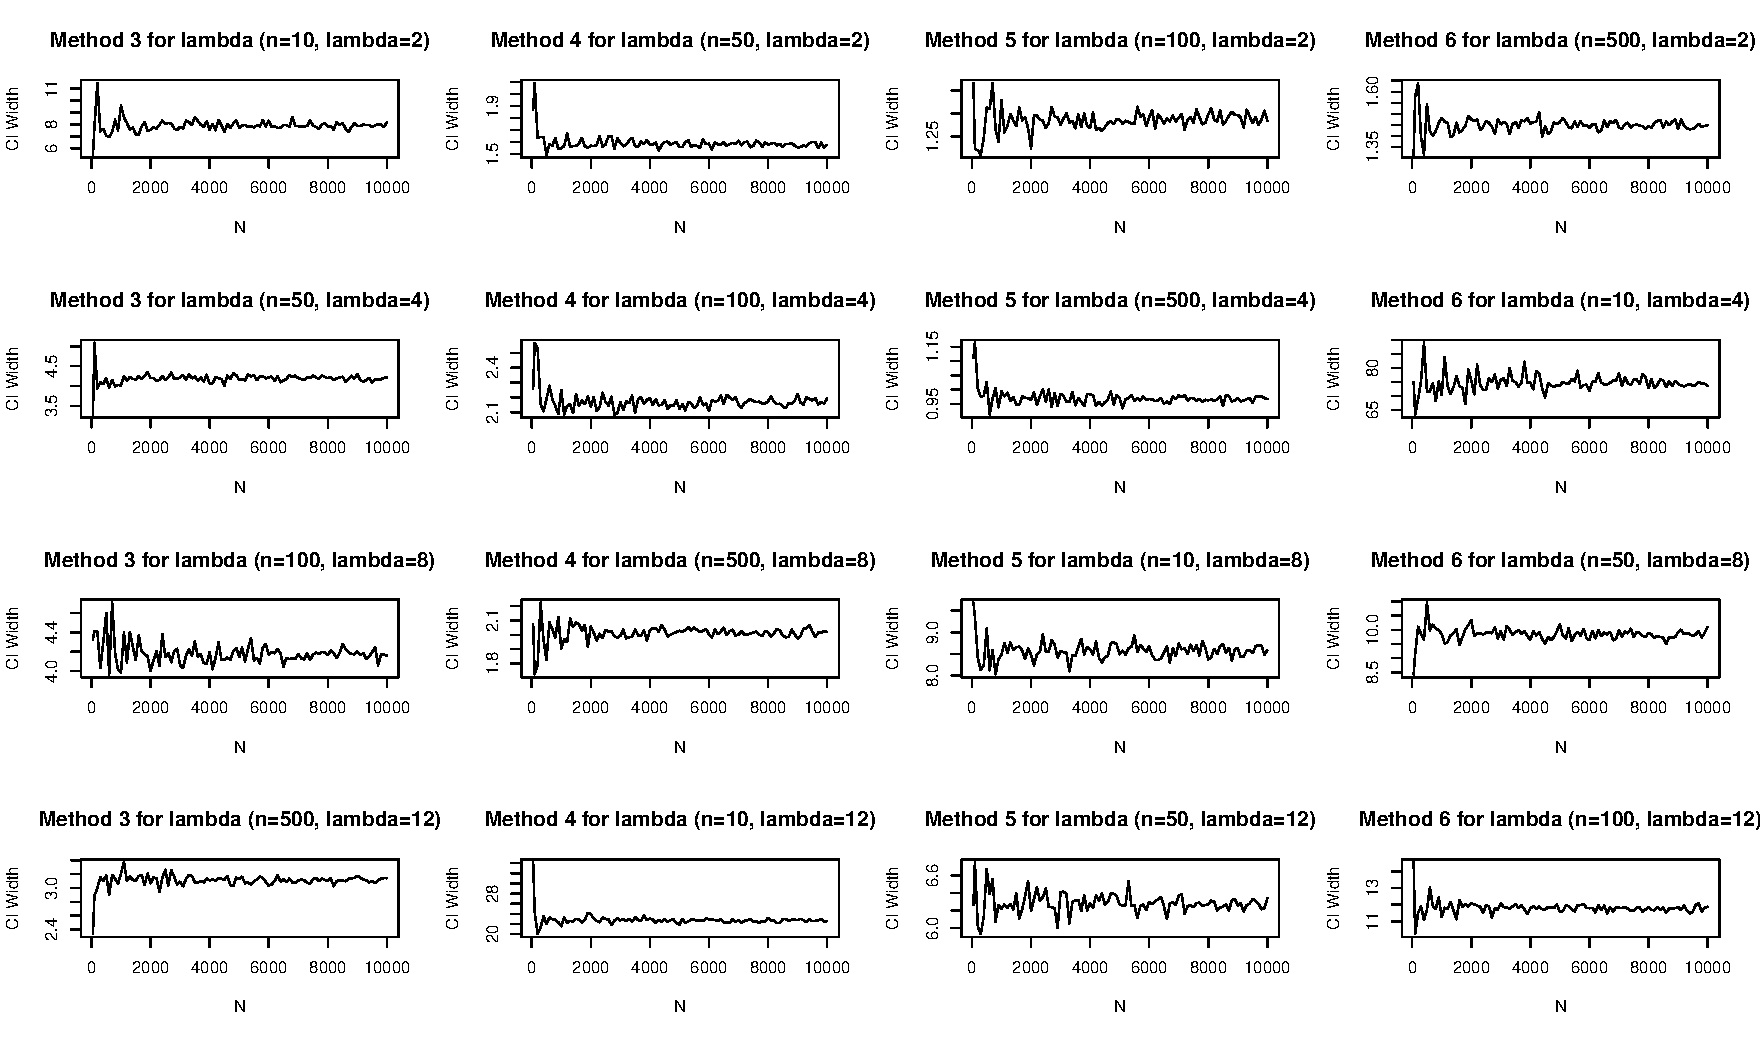
\includegraphics[width=1.0\textwidth]{findN_la.pdf}
\caption{Choose bootstrap N using the CI width of $\lambda$}
\end{figure}


\begin{figure}[h] 
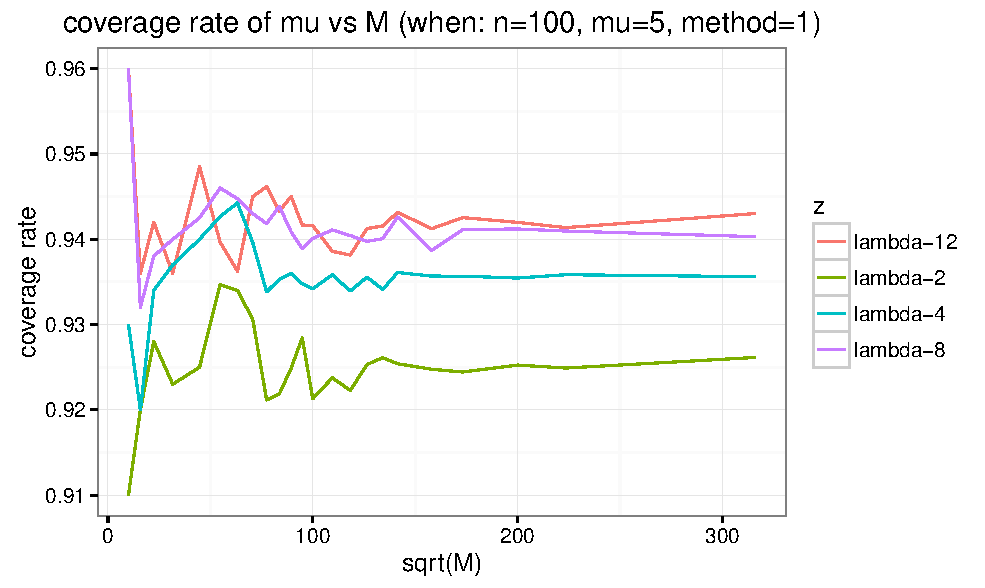
\includegraphics[width=0.8\textwidth]{findM1.pdf}
\caption{}
\end{figure}

\begin{figure}[h] 
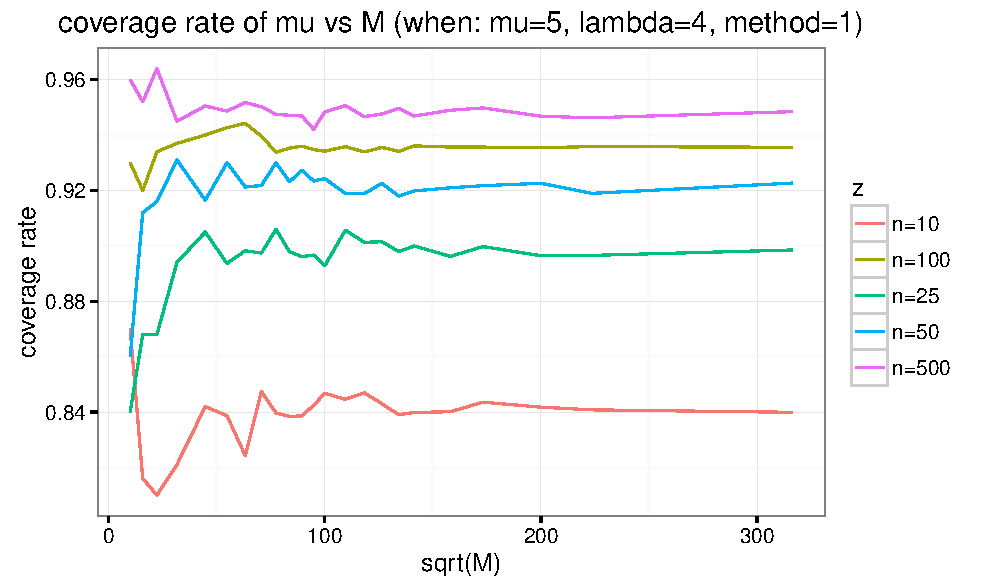
\includegraphics[width=0.8\textwidth]{findM2.pdf}
\caption{}
\end{figure}

\begin{figure}[h] 
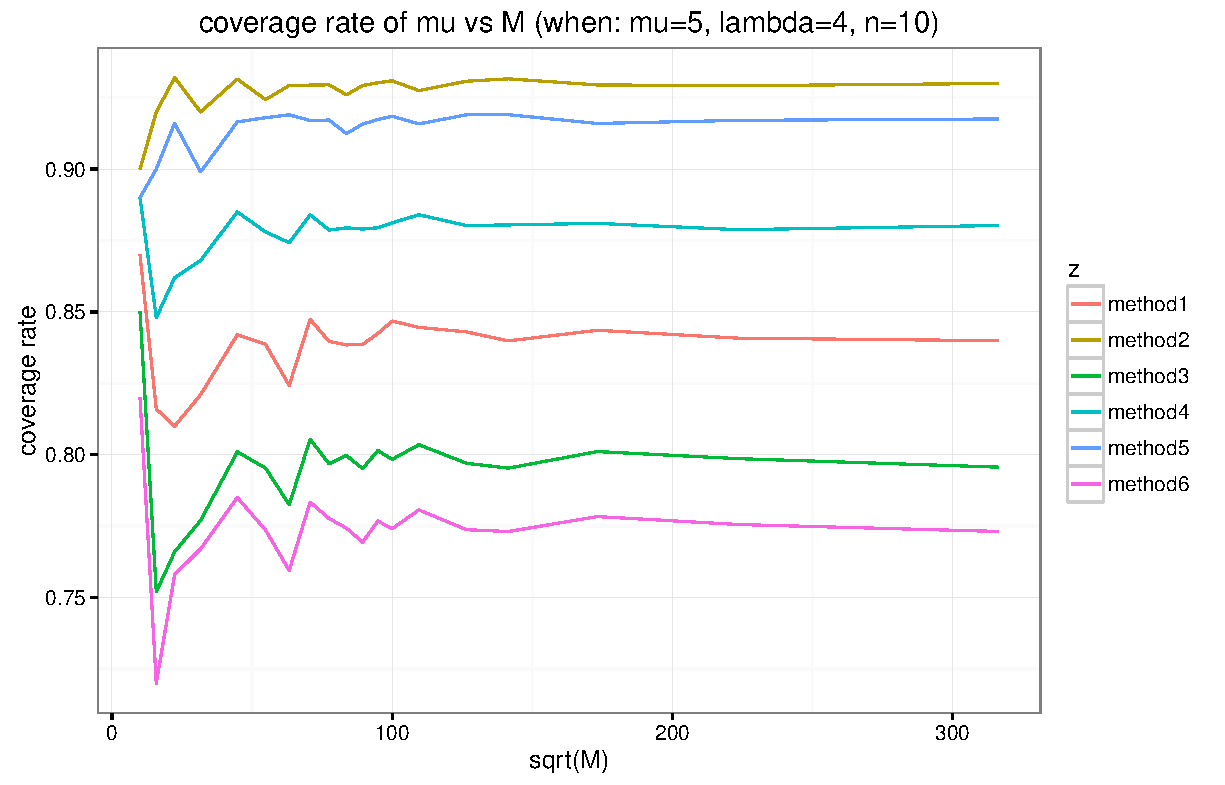
\includegraphics[width=0.8\textwidth]{findM3.pdf}
\caption{}
\end{figure}

\begin{figure}[h] 
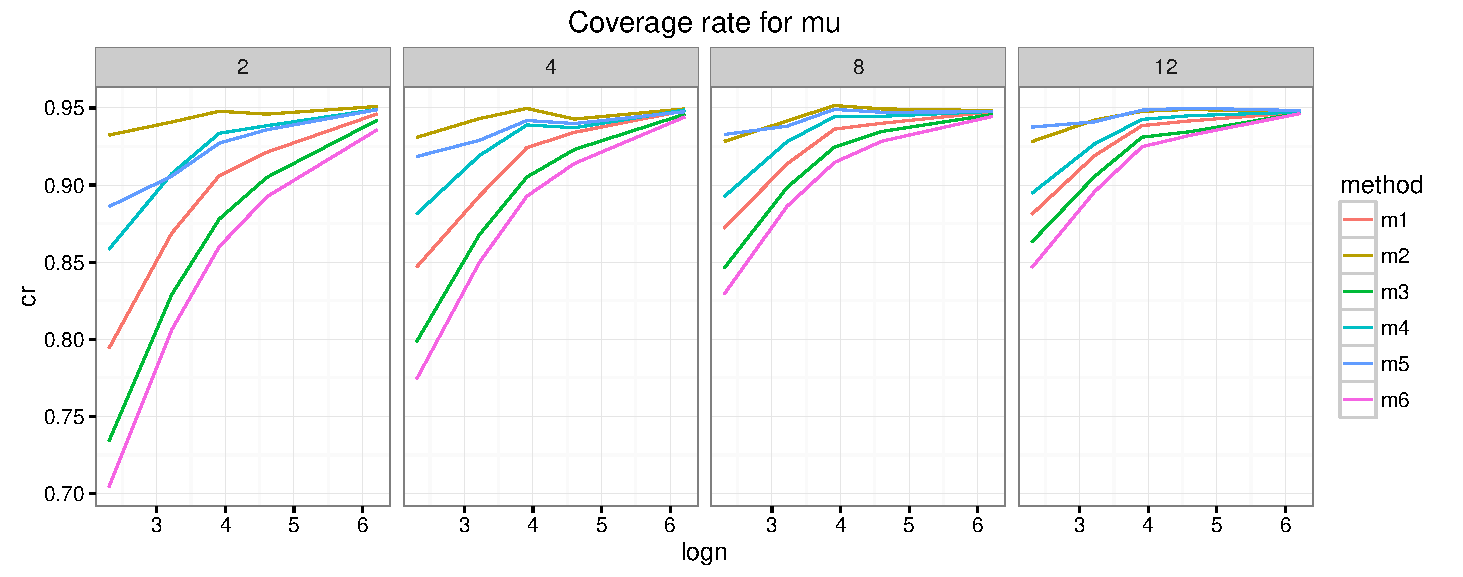
\includegraphics[width=1.1\textwidth]{results1.pdf}
\caption{}
\end{figure}

\begin{figure}[h] 
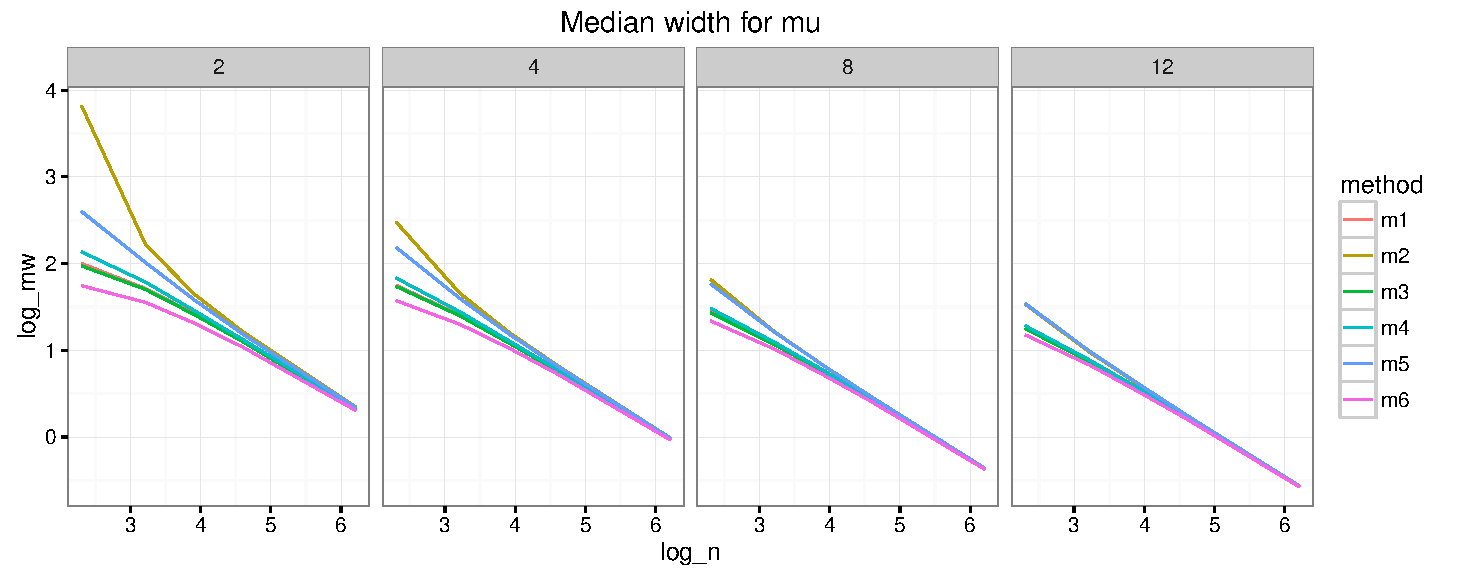
\includegraphics[width=1.1\textwidth]{results2.pdf}
\caption{}
\end{figure}

\begin{figure}[h] 
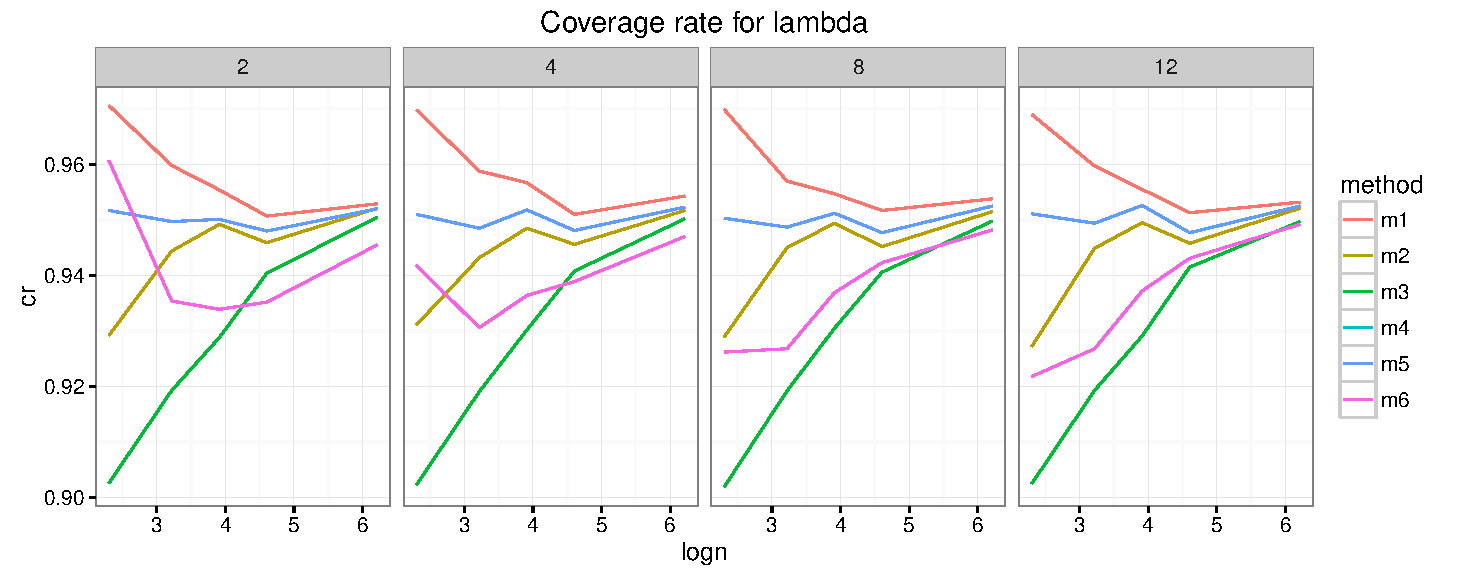
\includegraphics[width=1.1\textwidth]{results3.pdf}
\caption{}
\end{figure}

\begin{figure}[h] 
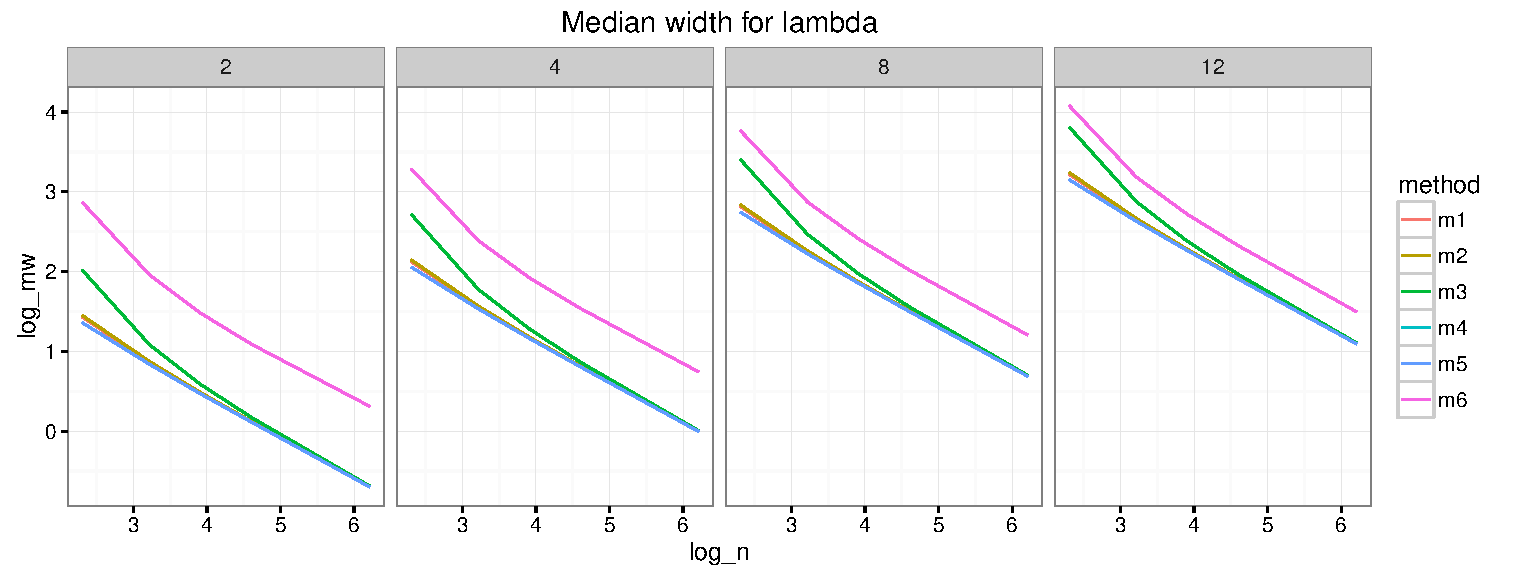
\includegraphics[width=1.1\textwidth]{results4.pdf}
\caption{}
\end{figure}


\begin{table}[h]
\csvautotabular{crmu.csv}
\caption{Coverage Rate for $\mu$}
\end{table}

\begin{table}[h]
\csvautotabular{crla.csv}
\caption{Coverage Rate for $\lambda$}
\end{table}

\begin{table}[h]
\csvautotabular{mwmu.csv}
\caption{Median Width for $\mu$}
\end{table}

\begin{table}[h]
\csvautotabular{mwla.csv}
\caption{Median Width for $\lambda$}
\end{table}

\begin{table}[h]
\csvautotabular{pmu.csv}
\caption{Out of Bound Probability for $\mu$}
\end{table}

\begin{table}[h]
\csvautotabular{pla.csv}
\caption{Out of Bound Probability for $\lambda$}
\end{table}



\end{document}